\documentclass[../Thesis_AHoecherl.tex]{subfiles}

\begin{document}
    \section{Allocation of initial margin}\label{Allocation of initial margin}
    The goal of this section is to investigate if a numerical Euler allocation of \gls{ISDA SIMM} is possible.
    
    As pointed out in section \ref{sec:Euler allocation} a risk measure needs to exhibit positive homogeneity of degree 1 to be able to perform an Euler allocation.
    In a first step we can investigate by calculating ISDA SIMM for a single trade whether ISDA SIMM does exhibit positive homogeneity for a minimal example.

    For this we set up an USD Libor IRS with ten years time to maturity and a notional of 200 billion USD. This is our initial portfolio $\mathbf{u}$. ISDA SIMM would fulfill the required positive homogeneity condition if $a \rho(\mathbf{u}) = \rho(a \mathbf{u}$ for $a>0$. In figure \ref{fig:homogeneity of ISDA SIMM} $\rho(a\mathbf{u})$ is plotted for $0<a\leq 2$ in blue. 
    \begin{figure}
        \centering
        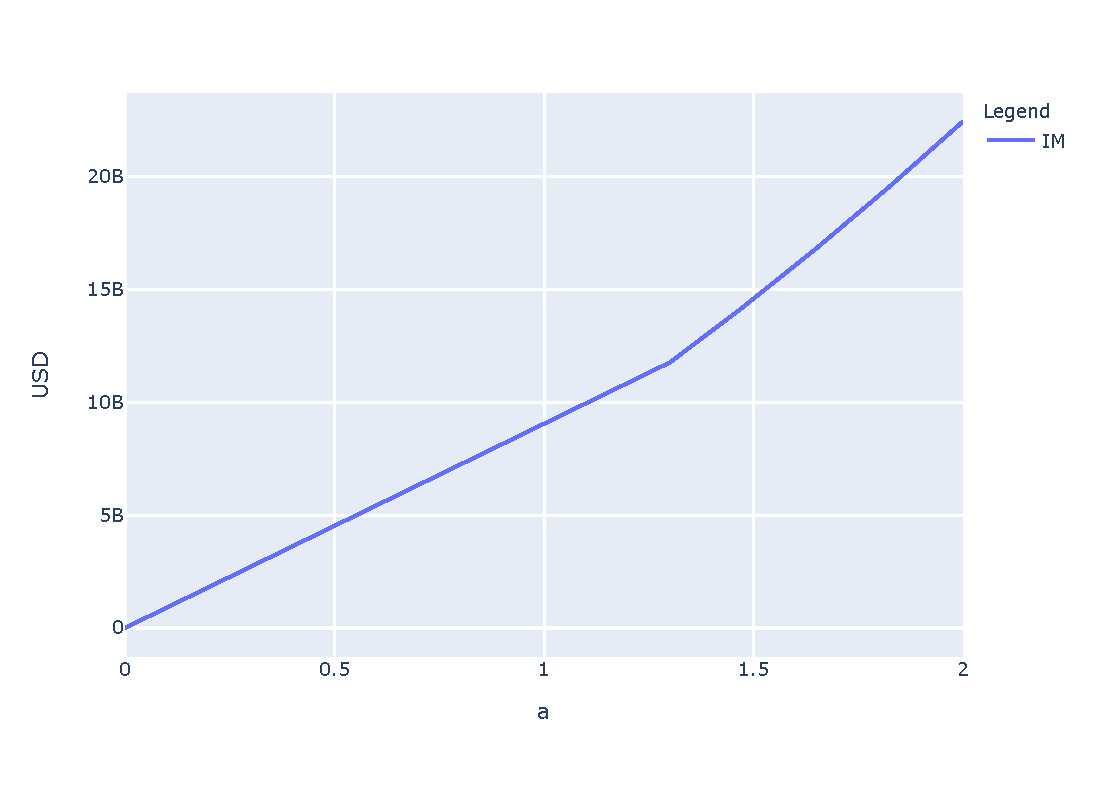
\includegraphics{Graphics/ISDA_SIMM_homogenity.pdf}
        \caption{}
        \label{fig:homogeneity of ISDA SIMM}
    \end{figure}
    The function exhibits homogeneity for $0<a<1.4$ \todo{find the exact point where homogeneity breaks} but not for higher $a$. 
    The reason for this is, that at this point the concentration risk charge of ISDA SIMM does kick in.
    The concentration risk for interest rate risks for our minimal example is defined as \cite[Article 7.b]{SIMM}
    \begin{align*}
        CR = \max\left(1,\left(\frac{\lvert\sum{s}\rvert}{T}\right)^{1/2}\right)
    \end{align*}
    with $s$ being the sensitivities against USD interest rate risk and T being 230Mn USD as specified in \cite[Article 74]{SIMM}. Due to subsequent variance-covariance aggregation the concentration risk impacts the calculated IM as
    \begin{align*}
        IM_{\text{with conc. risk}} = CR^2 \cdot IM_{\text{without conc. risk}}
    \end{align*}
    This causes the change in slope and implied loss of homogeneity visible in figure \ref{fig:homogeneity of ISDA SIMM}. If the portfolio would consist of a more diverse set of risk factors than the minimal example displayed in figure \ref{fig:homogeneity of ISDA SIMM} the associated concentration risk would kick in at different levels of $a$.
    The slope of the function would increase with each additional concentration risk not being floored at one any more. 
    
    It is important to note that as soon as the sensitivity against a single risk factor in the portfolio is above the concentration threshold the ISDA SIMM risk measure does not exhibit homogeneity anymore.

    Even a trivial example with just one trade is sufficient to show that Euler allocation does not work in the inhomogeneous part of the ISDA SIMM equation.
    For this, we compare two sample portfolios one consisting of one USD IRS with 200 bn notional and one consisting of one USD IRS with 400 bn notional.
    Critically, the second portfolio is penalized by the model since its USD IRS risk is too large. We calculate the Euler calculation with a forward finite difference approach as displayed in equation \ref{eq:forward difference}.

    Assuming that we calculate the finite difference with an $\epsilon = 0.0001$ this means that we calculate the ISDA SIMM of an IRS with 200Bn notional ($SIMM_{200Bn}$) and the ISDA SIMM of an equivalent IRS with 200.02 Bn notional ($SIMM_{200.02Bn}$) and this yields an Euler allocation to this trade as
    \begin{align*}
        \frac{SIMM_{200.02Bn} - SIMM_{200Bn}}{0.0001} = 9.04Bn
    \end{align*}
    We can see in figure \ref{fig:homogeneity of ISDA SIMM} that this value is both, the slope and the IM value at $a = 1$. The portfolios IM was correctly fully allocated to the single trade of which it consists. 
    
    However, performing the same calculation for an equivalent IRS with 400Bn notional yields
    \begin{align*}
        \frac{SIMM_{400.04Bn} - SIMM_{400Bn}}{0.0001} = 33.67Bn
    \end{align*}
    again, we can refer to figure \ref{fig:homogeneity of ISDA SIMM} to check if this is a reasonable allocation result. As $a=1$ represents the IM charge for investing 200Bn of notional in the IRS, $a=2$ represents an investment of 400Bn notional. The associated IM is just 22.44Bn - allocating 33.67Bn of the risk measure to the only trade in the portfolio is therefore clearly wrong. The Euler allocation of 33.67Bn can also be read off figure \ref{fig:homogeneity of ISDA SIMM} - it is the slope at $a=2$ times two.

    



    \section{Allocation of SA-CCR}\label{Allocation of SA-CCR}

    \subsection{Homogeneity of SA-CCR}

    \subsubsection{Homogeneity of C}

    To allocate \gls{SA-CCR} under consideration of margining, the available collateral $C$ is of special interest. As pointed out in table \ref{tab:Margin in SA-CCR} depending on the margining approach, C can be calculated as $C = \text{VM}$ or $C = \text{VM} + \text{IM}_{\text{received}}$.
    \begin{figure}
        \centering
        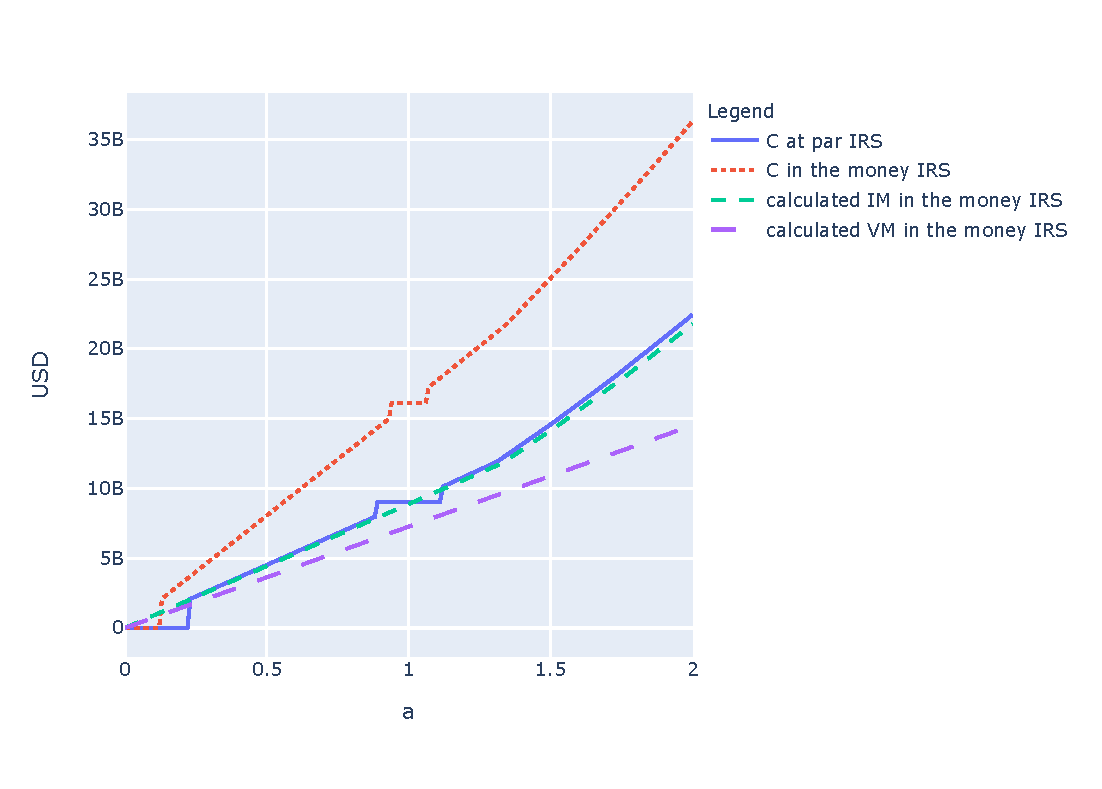
\includegraphics{Graphics/C_homogenity.pdf}
        \caption{}
        \label{fig:homogeneity of C}
    \end{figure}
    The actually exchanged collateral, however has to be calculated under consideration of the threshold and minimum transfer amount as displayed in equation \ref{eq:C}. With this consideration of threshold and minimum transfer amount $C$ is not a homogeneous function. 
    This can exemplary seen in \ref{fig:homogeneity of C}. This figure displays $C$ for an at the money 10Y USD interest swap and the same swap with a lower fixed rate making it an in the money swap. Again, a very high notional of 200 Bn is chosen to showcase the concentration risk charge of ISDA-SIMM and the threshold and minimum transfer amount have also been chosen to be very high at 2Bn and 1Bn USD.
    Figure \ref{fig:homogeneity of C} also showcases the trivial result that the Variation Margin is a homogeneous function - the value of the trade scales linearly with the notional.
    To be able to calculate an Euler allocation of SA-CCR one has to calculate C for use in \ref{eq:multiplier} without recognition of the minimum transfer amount as shown in equation \ref{eq:C no MTA}
    \begin{align}
        \label{eq:C no MTA}
        C_{\text{noMTA}} = \begin{cases}
            0  &\text{if } |C_{calc}|<\text{TH}\\
            C_{calc} &\text{oterhwise}
        \end{cases}
    \end{align}
    
    Again, similar to the exemplary calculation in section \ref{Allocation of initial margin} it can be shown with a trivial example, that Euler allocation of SA-CCR is not possible under recognition of a \gls{MTA}. 
    For this we consider the same 200Bn \gls{IRS} as in section \ref{Allocation of initial margin}. We assume that the currently posted margin is 9.04Bn which is the calculated ISDA-SIMM margin. 
    Setting $C$ at 9.04Bn in \ref{eq:multiplier} and then calculating the SA-CCR EAD for this single IRS \todo{as specified in ...} yields an regulatory EAD of 582.8Mn USD. Any natively additive allocation should allocate this full amount to the IRS.
    The \gls{VM} is zero as the IRS is struck at par.
    \begin{table}[htbp]
        \label{tab:Allocate SA-CCR with MTA calculation}
        \centering
            \begin{tabular}{c|c|c}
                & $\text{SA-CCR}_{\text{MTA}}$ & $\text{SA-CCR}_{\text{No \gls{MTA}}}$ \\
                \toprule
                Initial C & 9038.2Mn & 9038.2Mn \\
                \midrule
                EAD\textsubscript{200Bn IRS} & 582.8Mn & 582.8Mn \\
                \midrule
                C\textsubscript{200Bn IRS} & 9038.2Mn & 9038.2Mn \\
                \midrule
                C\textsubscript{200.02Bn IRS} & 9038.2Mn & 9039.1Mn \\
                \midrule
                EAD\textsubscript{200.02Bn IRS} & 583.0Mn & 582.9Mn \\
                \midrule
                $\frac{\text{EAD\textsubscript{200.02Bn IRS}}-\text{EAD\textsubscript{200Bn IRS}}}{0.0001}$ & 1425.3Mn & 582.8Mn  \\
            \end{tabular}%
        \caption{Numerical Euler allocation of SA-CCR with and without consideration of a minimum transfer amount for an example of a portfolio with a single 200Bn notional IRS. Euler allocation is only successful if the \gls{MTA} is not considered for the recalculation of the received margin C}
    \end{table}
    In table \ref{tab:Allocate SA-CCR with MTA calculation} we assume that the initially received collateral is the currently calculated collateral. 
    When calculating the Euler allocation with a forward difference in line with \ref{eq:forward difference} the received collateral when rising the notional to 200.02Bn increases when no MTA is assumed while it remains unchanged with consideration of an MTA. 
    Ultimately, this difference leads to a correct allocation of the entire EAD to the single IRS with the \emph{No MTA} approach while the \emph{MTA} approach obviously yields a wrong result by allocating 244\% of the portfolios EAD to its only trade.

    Critically, this result can also be transferred to any SA-CCR allocation approach that would treat C as an externally given constant value as locally, treating C as a constant value is the same as consideration of a \gls{MTA}. 
    In both cases the slope of C is zero. 
    
    Euler allocation of SA-CCR also does not work if the calculated C does not exhibit homogeneity, i.e. if a concentration risk threshold of the ISDA-SIMM model is exceeded. Again using the 400Bn IRS from \ref{Allocation of initial margin} we calculate an EAD\textsubscript{400Bn IRS} of 843.5Mn but, despite not applying an MTA, Euler allocation yields a vastly different amount of $ \frac{\text{EAD\textsubscript{200.02Bn IRS}}-\text{EAD\textsubscript{200Bn IRS}}}{0.0001} = 201.0Mn $. If for a given portfolio C does not exhibit homogeneity, neither does SA-CCR and therefore Euler allocation of SA-CCR is not possible for such portfolios.

    This implies the following important result:
    
    Euler allocation of SA-CCR is not possible if C is assumed to be constant $\neq 0$. C has to be a homogeneous function w.r.t. the position size and a possible minimum transfer amount has to disregarded for the calculation of the Euler allocation.

    Unlike the \gls{MTA}, the threshold should be taken into consideration when calculating an Euler allocation. 
    Inclusion of the threshold does not break the calculation of the Euler allocation, since both cases of equation \ref{eq:C no MTA} exhibit homogeneity in line with its definition \ref{eq:positive homogeneous function} for a certain range around $a$. 
    Numerical calculation of the Euler allocation only malfunctions due to inclusion of the threshold if $C(1) = 0$ but $C(1+\epsilon) = C_{\text{calc}}$ \todo{notation (1), (1+epsilon) needs to be refinded}.

    \subsubsection{Euler allocation of hedge trades}

    As pointed out in \ref{Allocation of Risk Measures} Euler allocation is a risk sensitive allocation and as such does generally attribute negative contributions to trades that are decreasing the risk of the portfolio. If we consider a portfolio of a 200Mn payer IRS, an equivalent 100Mn receiver IRS and 1Mn long stock call options we yield the result depicted in \ref{tab:hedge trade sample results} when calculating the Euler allocation numerically with a forward difference.

    \begin{table}[htbp]
        \label{tab:hedge trade sample results}
        \centering
            \begin{tabular}{c|c|c}
                & SA-CCR & ISDA SIMM \\
                \toprule
                IRS\textsubscript{100Mn Rec} & -246k & -4.52Mn \\
                \midrule
                IRS\textsubscript{200Mn Pay} & 493k & 9.04Mn \\
                \midrule
                Equity Option & 1.30Mn & 6.95Mn \\
                \bottomrule
                Sum of allocations & 1.54Mn & 11.47Mn \\
                \midrule
                Portfolio risk measure & 1.54Mn & 11.47Mn \\
            \end{tabular}%
        \caption{}
    \end{table}

    \begin{table}[htbp]
        \label{tab:EAD perfect hedge}
        \centering
            \begin{tabular}{c|c|c|c}
                & Forward & Central & Backward \\
                \toprule
                IRS\textsubscript{200Mn Rec} & 188k & 0k & -188k \\
                \midrule
                IRS\textsubscript{200Mn Pay} & 188k & 0k & -188k\\
                \midrule
                Equity Option & 1.32Mn & 1.32Mn & 1.32Mn\\
                \bottomrule
                Sum of allocations & 1.69Mn & 1.32Mn & 944k \\
                \midrule
                Portfolio risk measure & \multicolumn{3}{c}{1.32Mn} \\
            \end{tabular}%
        \caption{}
    \end{table}

    \begin{table}[htbp]
        \label{tab:IM perfect hedge}
        \centering
            \begin{tabular}{c|c|c|c}
                & Forward & Central & Backward \\
                \toprule
                IRS\textsubscript{200Mn Rec} & 4.52Mn & 0.00Mn & -4.52Mn \\
                \midrule
                IRS\textsubscript{200Mn Pay} & 4.52Mn & 0.00Mn & -4.52Mn \\
                \midrule
                Equity Option & 6.95Mn & 6.95Mn & 6.95Mn \\
                \bottomrule
                Sum of allocations & 15.99Mn & 6.95Mn & -2.09Mn \\
                \midrule
                Portfolio risk measure & \multicolumn{3}{c}{6.95Mn}  \\
            \end{tabular}%
        \caption{}
    \end{table}

    \subsection{Allocation without margining}
    \subsection{Allocation under VM collateralization}
    \subsection{Allocation under VM and IM collateralization}
\end{document}